\documentclass[../main.tex]{subfiles}

\begin{document}
Like many other fields dealing with the classification of images, the DNN revolution impacted Facial Expression Recognition (FER).
This field can benefit from both major DNN architectures. The CNN - enabling a better understanding of image data through learned features.
The RNN - enabling a better understanding of temporal relationships in time series data.
In this section, we review a few studies in the field that we feel best suit our project's goals.
\par

A recent study in the field \cite{emotionnet-nano} attempted to create a very efficient model that would be able
to recognize facial expression while running on an embedded device.  EmotionNet Nano, the model introduced in the paper,
was constructed with a similar philosophy to EfficientNet \cite{effnet}. The authors started with a base model and then defined an
optimization problem to maximize the model's accuracy while constraining it to a size of less than 1M parameters.
As described in the paper, the use of automatic network design exploration provided a significant advantage over hand-crafted
designs in its ability to produce very heterogeneous blocks that better fit the problem.
As we can see from the model architecture \ref{fig:emotionnet_nano}, two fascinating phenomena exist in this model:

 
\begin{itemize}
    \item We can see that the layers' shapes differ from one to another, increasing and decreasing the number of filters through the network.
    \item The residual connections are not the same for each layer and even skip some layers entirely.
        This phenomenon is referred to in the paper as selective long-range connectivity. The model generator's ability to choose such
        specific residual connections creates a healthy balance between model expressiveness and ease of training.
    \item Maybe most interesting are the 1x1 convolution layers that tale outputs from multiple 3x3 convulsions
        and connect back to the network at deeper layers. These connections provide dimensionality reductions and retain older
        features by mixing the channels, meaning the model's expressiveness is increased for a low computational cost.
\end{itemize}
 

We chose to focus on this paper because of the model's simplicity combined with its state of the art performance. In the paper,
the authors present two models. One smaller and less accurate model, achieving 92\% accuracy on CK+,
and the other slightly bigger achieving 97\% accuracy on CK+. The "Big" model only has ~200k parameters, meaning it would be effortless to
train and experiment with it. The other reason is its performance. Though the authors optimized the model for inference performance,
its size means that it will be relatively light to train, which is vital for our use case of perpetual training personalized model.
We will discuss our experiments in more depth in the experiments section, though this model will allow us to retrain it on different data
with different labels and even make adjustments to the model quickly, which is also very important to us.
\par

\begin{figure}[htp]
    \centering
    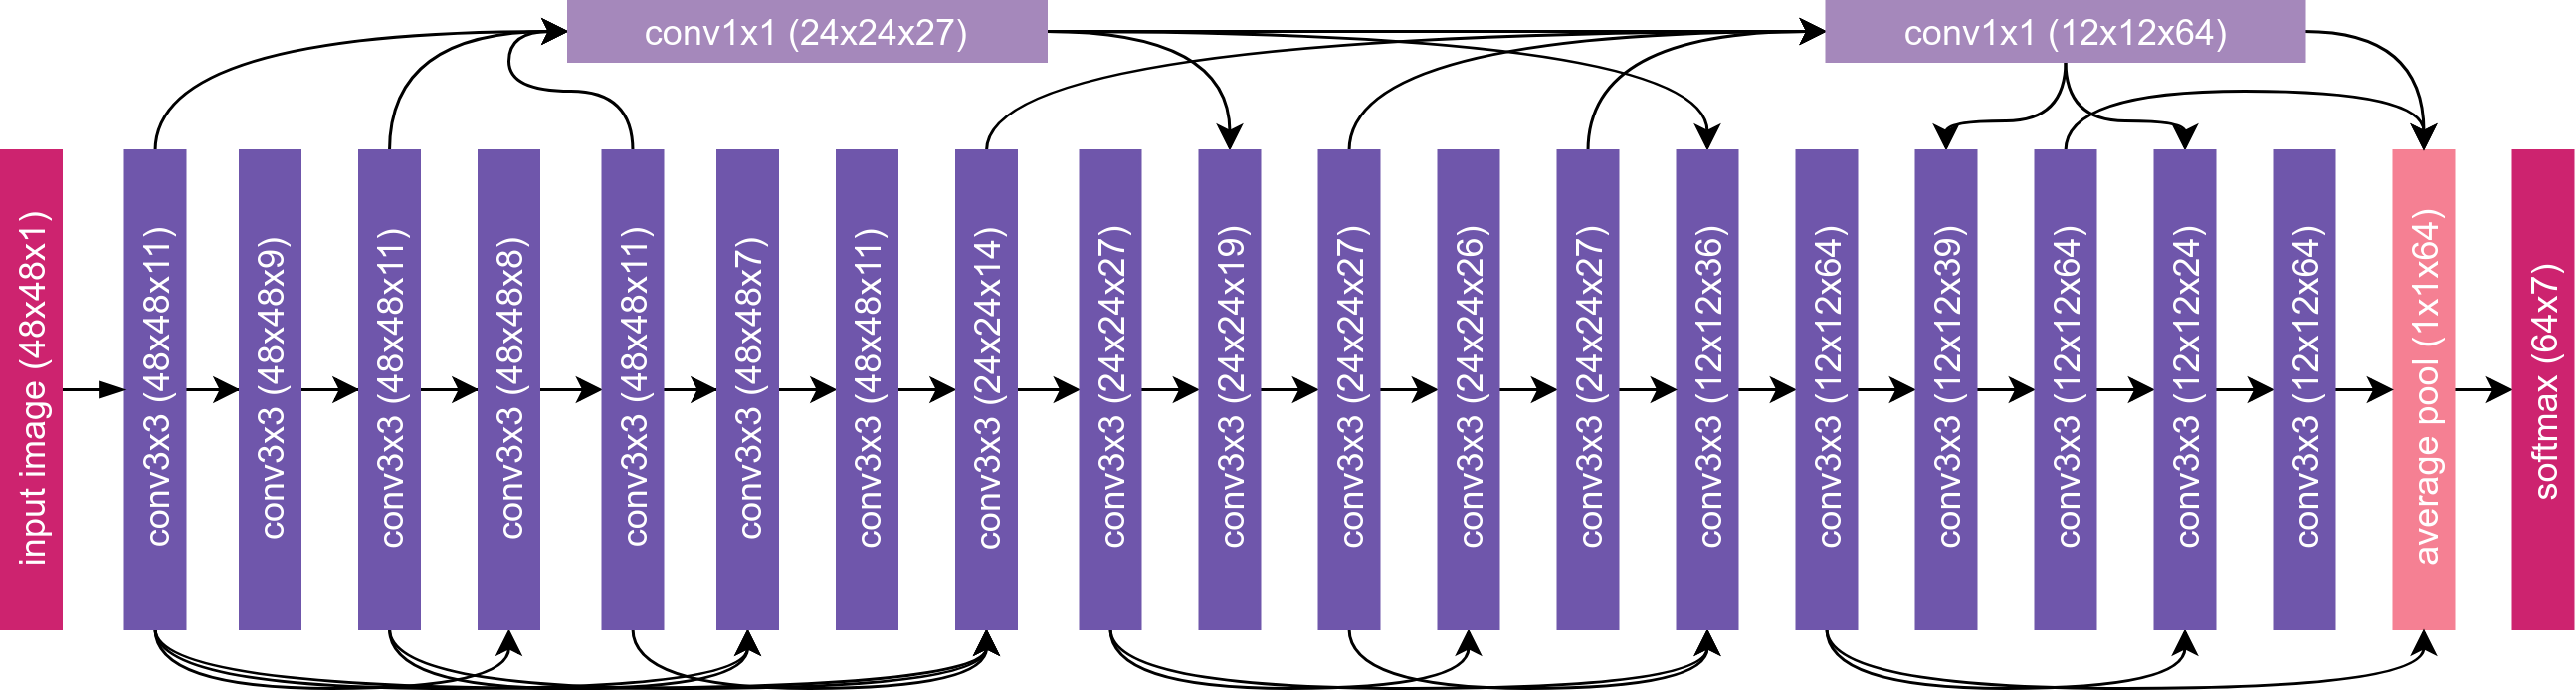
\includegraphics[width=12cm]{figures/emotionnet_nano.png}   
    \caption{EmotionNet Nano architecture as shown in the paper \cite{emotionnet-nano}}
    \label{fig:emotionnet_nano} 
\end{figure}

One significant improvement to models such as EmotionNet Nano is the addition of temporal information when classifying emotions.
Facial Expressions are very dynamic, meaning that information from only one frame can be misleading to the overall emotional state of the subject.
We can easily imagine a situation where, in three different frames, the subject expresses three different emotions according to a static model,
and we would have to learn a more general representation of emotion using the surrounding frames.
Meng et al. \cite{fan} explore this idea by creating a two-stage model. The first stage of the model is very straightforward.
It uses a pre-trained ResNet model to create the image embeddings for each frame. The innovative part of the model is in the second attention stage.
The embeddings are transformed through 4 steps into the final video representation on which softmax is activated to output the label.

 
\begin{enumerate}[i]
    \item The embeddings $f_i$ flow through a fully connected layer, generating the attention weights for the images - $\alpha_i = \sigma(f_i^Tw_i^0)$
        where $\sigma$ is the activation function, and $w_i^0$ are the weights of the FC layer.
    \item All the attention weights are summed up to create the video context representation - $c'=\frac{\sum_{i=1}^{n}\alpha_if_i}{\sum_{i=1}^{i=n}\alpha_i}$
    \item Next, we concatenate the context $c'$ to each of the original embeddings - $[f_i:c']$, and calculate the second attention weights, this time 
        taking into account both the original features and the overall video representation - $\beta_i = \sigma([f_i:c']^Tw_i^1)$
    \item Finally, we sum up all the attention weights to get the final representation of the video - 
    $c = \frac{\sum_{i=1}^{n}\alpha_i\beta_i[f_i:c']}{\sum_{i=1}^{i=n}\alpha_i\beta_i}$
\end{enumerate}
 

In the paper, the first two steps are referred to as self-attention, and the last two steps are called relation-attention.
This combination of the more traditional self-attention approach and the so-called relation-attention, enables a much more refined network.
The authors claim that using both attention layers makes the network more reliable because the attention is not only based on the individual frame,
which can cause the network to be biased towards higher or lower emotions in specific places in the video. Instead, the attention combines the basic frame
features with the whole video representation. This way, the attention can be based on the frame's relation to the video.
On the other hand, we can see from the results that the improvement gained from using the second attention layer is relatively small. On the CK+ dataset,
the second attention layer improved the results from 99.08\% to 99.69\%. We intend to compare the performance-cost tradeoff of
using the second layer with our model, where the results might differ.
\par

There are many more ways of tackling this problem, but we would like to focus on an older method \cite{c3d},
though the results are not comparable to the other two methods as EmotionNet Nano \cite{emotionnet-nano} is only tested on CK+ and FAN \cite{fan}
is tested on the same dataset but only compares with single network solutions. We can see that the solution proposed in Fan's et al. work \cite{c3d}
has at least comparable performance as it achieves 56\% accuracy with its smallest model, compared to 51\% for FAN \cite{fan}.
Regardless we found the methods proposed in Fan's et al. work \cite{c3d} unique and worth exploring in our research.
\par

Fan et al. \cite{c3d} proposes an ensemble made up of three separate models. Similarly to FAN \cite{fan},
the first model takes a pre-trained VGG model and applies "temporal analysis" to the embedding generated. In this case,
an LSTM \cite{lstm} layer is used, meaning that each embedding needs to go through the model in order, and only the result of the final frame will
continue to the next stage. The second model is a simple convolutional network except that the filters are three dimensional instead of
the two-dimensional filters usually applied to 2D images. Such filters are often used when working with 3D objects as their output is also a 3D tensor.
In this model, the input is a "3D shape", made up of a series of images, and the 3D convolutions allow the network to keep the time dimension intact
and represent the temporal relationships between the images as an additional spatial dimension on which the network can convolve. The third model
is a simple SVM trained on audio.
\par

We will not experiment with audio as an additional input for our models, but facial models combined with none image data are already encouraging.
Though we will attempt an ensemble using keyboard and mouse inputs instead of audio, the paper's ensemble method is still relevant. In the paper,
the models are weighted according to their performance. The model's results are fused by weighted summation to produce the final prediction. 
\par

Finally, we note some of the properties of the Conv3D model. First, we have a unique way of dealing with the temporal dimension since the model
has no unique representation for the time dimension, which is treated as just another spatial dimension.
This can cause mixing of the features along the time dimension, which could be positive if we consider that the model can generate temporal
features along part of the image, which is impossible in other methods. On the other hand, the model could confuse time and generate features
that mix frames from different times in an incorrect order. This method also requires that all the frames have the same augmentations applied
to them so that the video would be fluid. If the video is augmented frame by frame,
it could cause the frames to be inconsistent and create wrong temporal features.



\end{document}